\documentclass[a4paper,10pt]{article}
\usepackage[utf8]{inputenc}
\usepackage{amssymb,amsmath}
\usepackage{graphicx}
\graphicspath{{../images/}}

%opening
\title{}
\author{}

\begin{document}

\maketitle

\begin{abstract}

\end{abstract}

\section{Overview of Machine Learnnig}
\begin{enumerate}
 \item Logistic Classification
 \item Stochastic Optimization
 \item Data and Parameter Turning
 \item Deep Networks
 \item Regularization
 \item Convolutional Networks
 \item Embeddings
 \item Recurrent Models
 
\end{enumerate}


\section{History of Neural Networks}
\begin{enumerate}
 \item Fukushimas Neocognitron - 1980's
 \item Lecun's Net -1990
 \item Krizhevsky's Alexnet
 \item Speech Recognition -2009
 \item Computer Vision -2012
 \item Machine Translation - 2014
 
\end{enumerate}

\section{Classification}

Given set of images and labels in training data. In test data completely new image comes. Classify image. After classification we can do 
\begin{enumerate}
 \item Regression
 \item Ranking - In web page. Classify relevant or irrrelevant
 \item Reinforcement Learning
 \item Detection  - Eg : Detect presence or absence of pedestrian
\end{enumerate}


\subsection{Logistic Classifier}

\begin{equation}\label{linear}
 WX +b =Y
\end{equation}
  
 X - Image Pixels \\
 Y - Labels\\
 W- Weight\\
 b- Bias\\
\subsubsection{Soft Max Function}

Softmax function converts scores into probability
\begin{equation}
 S(y_i) = \frac{e^y_i}{\displaystyle \sum e^y_j}
\end{equation}


\subsubsection{One Hot Encoding}

One for correct class and zero to other class labels.

\subsubsection{Cross Entrophy}

The way to measure distance between two probabilities is called cross entrophy.

\begin{equation}
 D(S,L) = -\displaystyle \sum_i L_i log(S_i) 
\end{equation}

Cross Entrophy is not symmetric. $D(S,L) \neq D(L,S) $\\

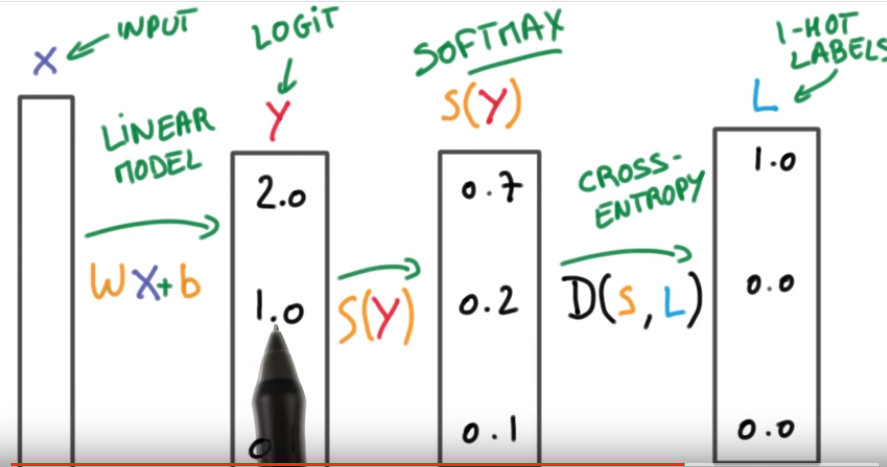
\includegraphics[width=10cm, height=5cm]{nnend2end}
\section{Training Loss}

Loss = Average Cross entrophy. We do  to minimize distance between similar labels and maximize distance between dissimilar labels.

\begin{equation}
 L=\frac{1}{N}{\displaystyle \sum_i D(S(WX_i + b),L_i) }
\end{equation}


\section{Gradient Descend}

While taking average to calculate training loss we are taking average of distance between probabilities. Gradient descend for two weights is calculated as follows.


\begin{equation}
 Gradient Descent for weight w_1 and w_2 = \Delta L(w_1,w_2)
\end{equation}


But in real-time the weight is computed for all parameters.


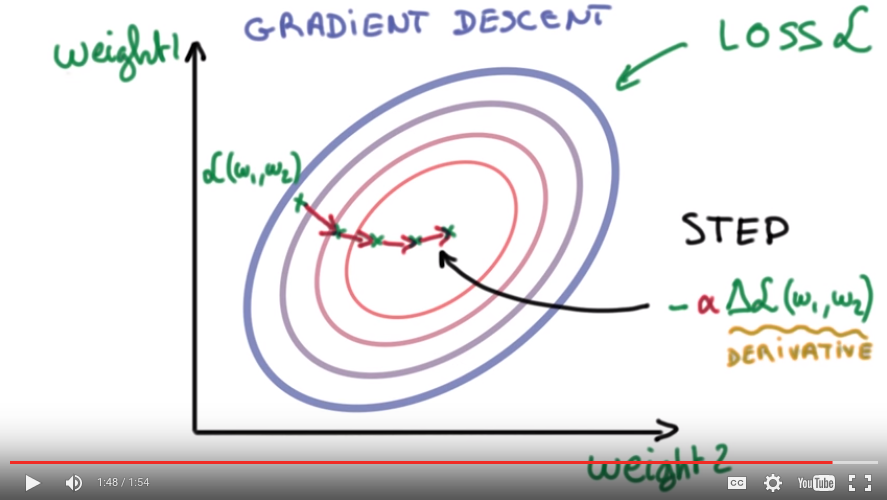
\includegraphics[width=10cm, height=5 cm]{gradientDescend}
\subsection{Big Loss Function because of Numerical Unstability}

To overcome Big Loss function keep mean zero and equal variance.
\b Mean

\begin{align*} 
 X_i =0 
 \end{align*}

\b Variance

\begin{align*}
 \sigma(X_i) = \sigma(X_j)
\end{align*}

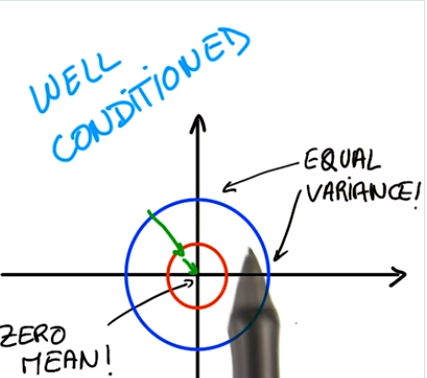
\includegraphics[width=5cm, height=5cm]{zeromean}

\subsection{Normalize Input for Gradient Descend}

To normalize pixel input normalize as follows.

\begin{align*}
\frac{R-128}{128} \qquad	\frac{G-128}{128}	\qquad \frac{B-128}{128}
\end{align*}

\subsection{Initialize Weight for Gradient Descend}

Initialize $w_0, b_0$



Large  value of $\sigma$ - Distribution has large peaks \\
Small value of $\sigma$ - Distribution is very uncertain.

Start with very small value of $\sigma$

 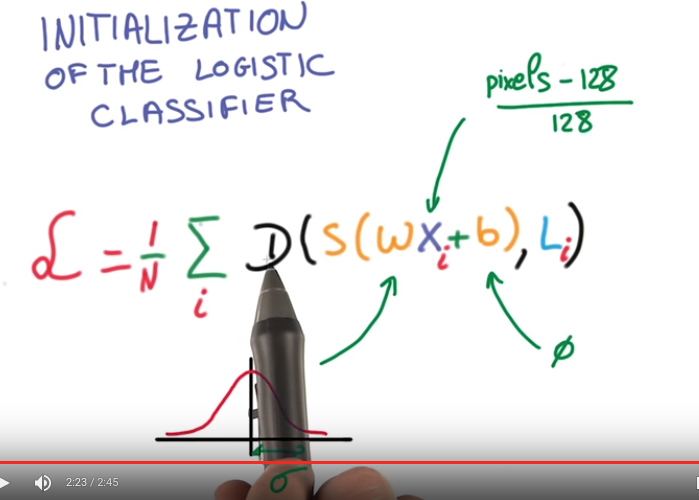
\includegraphics[width=5cm,height=5cm]{initializelogicclassifier}
 \subsection{Steps to Train Logistic Classifier}
 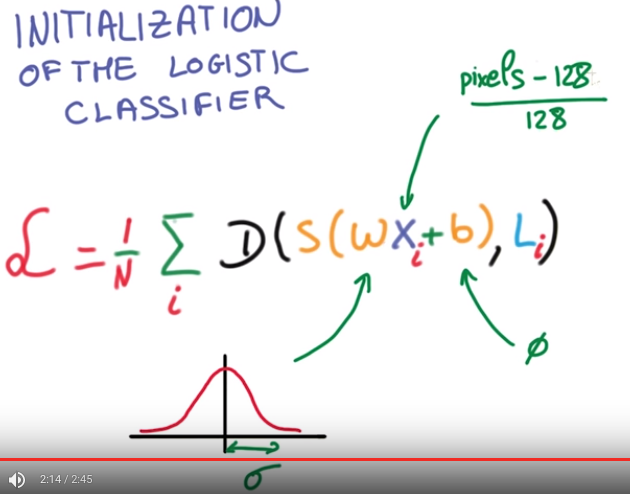
\includegraphics[width=10cm, height=5cm]{trainlogicclassifier}
 
 \begin{enumerate}
  \item $X_i$ - Training data is normalized to zero mean and equal variance
  \item w - Initialized with random weights
  \item Do softmax
  \item Do cross entrophy loss
  \item calculate average for entire training data
  \item Optimization - Compute derivative loss function w.r.to weight
   \item Optimization - Compute derivative loss function w.r.to bias
   \item derivative is in opposite direction (-)
   \item Loop through derivative function till we reach minimum of loss function.
 \end{enumerate}

 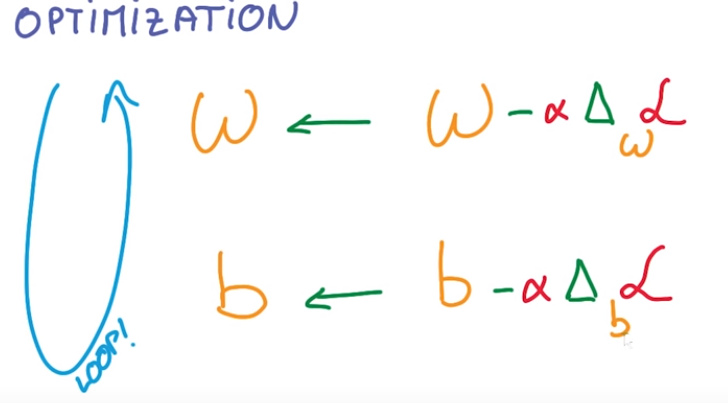
\includegraphics[width=10cm, height=5cm]{lcoptimize}
\end{document}
